\documentclass[10pt, a4paper]{article}
\usepackage[utf8]{inputenc}
\usepackage[frenchb]{babel}
\usepackage[OT1]{fontenc}
\usepackage{amsfonts, amsmath, amssymb, amsthm, dsfont, amsthm}
\usepackage{a4wide}
\usepackage[dvipsnames]{xcolor}
\usepackage{tikz} 
\usetikzlibrary{arrows,positioning,shapes}

\title{\textbf{Lab Report} \\ Week of 12/01/2016}
%\author{Olivier \textsc{Mangin}}
%\date{\today}

\definecolor{main}{named}{BurntOrange}
\definecolor{second}{named}{RoyalBlue}
%\newcommand{\maincolor}{orange}
%\newcommand{\secondcolor}{orange!20}
\newcommand{\strong}[1]{\textcolor{main}{\textbf{#1}}}
\newcommand{\stronger}[1]{\textcolor{second}{\textbf{#1}}}
\newcommand{\colored}[1]{\textcolor{main}{#1}}

% Affichage du titre avec les numéro et date de la semaine
\newcommand{\titre}[2]{
\noindent
\hspace{-10pt}
\begin{tabular}{lr}
  \hspace{0.58\textwidth} & \hspace{0.4\textwidth} \\
  \strong{\huge Lab Report} & \textbf{\Large #1} \medskip \\
  \textbf{\Large Name \& Roll} & {\large #2} ~\\
\end{tabular}

\vspace{20pt}
}

% Encadré ``En bref'' réumant les avancées et problèmes de la semaine
\newenvironment{enbref}{
\noindent\fcolorbox{main}{main}{
\begin{minipage}{\textwidth}
\textcolor{white}{\textbf{\large }}
\end{minipage}
} \\

}{
\begin{center}
  \strong{ \rule[2mm]{\textwidth}{3pt} }
\end{center}
\vspace*{-20pt}
}

% Affichage d'un titre de rubrique
\newcommand{\rubrique}[1]{
  \bigskip
  \begin{center}
  \begin{minipage}{\textwidth}
    \noindent\strong{{\large #1} \\
      \rule[2mm]{\textwidth}{1pt} }
  \end{minipage}
  \end{center}
  \vspace*{-20pt}
}

% Symbole utilisé en début de ligne des éléments
\newcommand{\doublerect}{
\begin{tikzpicture}
  \fill[color=main] (0,0) rectangle (4pt,-4pt);
  \fill[color=second] (2pt,-2pt) rectangle (6pt,-6pt);
\end{tikzpicture}
}

% Affichage d'un titre d'élément
\newcommand{\element}[1]{
  \medskip
  \noindent\textcolor{second}{ \doublerect \textbf{#1}}
}

% Pour les lectures, petit raccourci pour mettre en avant le niveau
% de lecture d'un article.
\newcommand{\lu}{\strong{[Lu]} }
\newcommand{\parcouru}{\strong{[Parcouru]} }
\newcommand{\alire}{\strong{[A lire]} }
\newcommand{\presentation}{\strong{[Présentation]} }
\newcommand{\keynote}{\strong{[Keynote]} }



\usepackage[pdfauthor={Name}, pdftitle={Weekly}, pdfsubject={Week 1}, pdfkeywords={},colorlinks=true,urlcolor=black,linkcolor=black, citecolor=black]{hyperref}
\usepackage{listings}
\usepackage{subfig}
\usepackage{graphicx}
\lstset{%
language=Matlab,
frame=single,
%numbers=left,
%numberstyle=\footnotesize,
%tabsize=2,
keepspaces=true,
columns=fullflexible,
basicstyle=\ttfamily\scriptsize,
keywordstyle=\color{blue}
}


\begin{document}

\renewcommand{\labelitemi}{\textcolor{main}{\small $\blacktriangleright$}}
\renewcommand{\labelitemii}{\textcolor{second}{\scriptsize \textbullet}}

\titre{Week 3}{05/01/2017}

\begin{enbref}
\element{Title}
\begin{itemize}
\item Draw a circle in OpenGL and Matlab using:\\
1). Bresenham’s mid-point circle Drawing Algorithm
\end{itemize}
\medskip

%\element{Problèmes rencontrés}
%\begin{itemize}
%\item Néant.
%\end{itemize}
\end{enbref}

%\rubrique{Lectures}
%Néant.
%\element{\lu ... \cite{...}}

\rubrique{Procedure}
\vspace{0.5mm} \flushleft

\element {OpenGL}

\vspace{0.5mm} \flushleft
1). Draw a circle using Bresenhams mid point Algorithm.
\begin{itemize}
\item Create a C file and name it as \textit{circleBresenhams.c}.

\item Define global variables to store coordinates of center and radius of a circle .

\item Following is the Bresenham Algorithm to draw circle in 1st octant:

\begin{lstlisting}
while x < y
	if (d < 0)
	   d += 4*x + 6;
	else 
	   d += 4*(x-y) + 10;
	   y--;
	end
	x++;
end \\


extend this to other octants. please see code
\end{lstlisting}

\item Following is the final code for Bresenhams circle drawing algorithms:
\begin{lstlisting}
#include <stdio.h>
#include <math.h>
#include <GL/glut.h>

int centre_x = 0 ; int centre_y=0 ; int radius =0 ;
int n = 0 ;
int x_coordinate[1000];
int y_coordinate[1000];

void displayCircle(void)
{
	glClear(GL_COLOR_BUFFER_BIT);
       
        int d = 3-2*radius;
	int x = 0, y = radius; 
	putPixels(centre_x, centre_y, x, y);
	
	while (x < y)
	{
		if (d < 0)
		{
		   d += 4*x + 6;
		}
		else 
		{
		   d += 4*(x-y) + 10;
		   y--;
		}
		x++;
		putPixels(centre_x, centre_y, x, y);
	}
    	int i;
    	for (i = 0; i < n; i++ )
    	{
		glBegin(GL_POINTS);
		glColor3f(1.0, 1.0, 1.0);
		//printf("x : %d y : %d\n", x_coordinate[i], y_coordinate[i]);
		glVertex2f(x_coordinate[i]/100.0, y_coordinate[i]/100.0);
		glEnd();
	}
    	glFlush();
}

void putPixels(int X, int Y, int P, int Q )
{
	x_coordinate[n] = X + P;
	y_coordinate[n++] = Y + Q;

	x_coordinate[n] = X - P;
	y_coordinate[n++] = Y + Q;

	x_coordinate[n] = X + P;
	y_coordinate[n++] = Y - Q;

	x_coordinate[n] = X - P; 
	y_coordinate[n++] = Y - Q;

	x_coordinate[n] = X + Q;
	y_coordinate[n++] = Y + P;

	x_coordinate[n] = X - Q; 
	y_coordinate[n++] = Y + P;

	x_coordinate[n] = X + Q; 
	y_coordinate[n++] = Y - P;

	x_coordinate[n] = X - Q;
	y_coordinate[n++] = Y - P;
}
int main(int argc, char const *argv[])
{
	printf("centre coordinates : ");
	scanf("%d  %d", &centre_x , &centre_y);
	printf("radius of circle   : ");
	scanf("%d",&radius);

	glutInit(&argc, argv);
        glutInitDisplayMode(GLUT_RGB);
        glutInitWindowSize(640,480);
        glutCreateWindow("Bresenham Circle Drawing Algorithm");
        glutInitWindowPosition(100,100);
        glutDisplayFunc(displayCircle);
        glutMainLoop();
	return 0;
}
\end{lstlisting}

\vspace{0.5mm}

\item Compile and run the executable file in terminal by typing in the following commands : \\

\vspace{0.5mm} \flushleft

\textit{(a)\hspace{2mm} gcc circleBresenhams.c -lGL -lGLU -lglut -lm} \\
\textit{(b)\hspace{2mm} ./a.out}
\vspace*{1\baselineskip} 
\end{itemize}

\element {MatLab}\\

1). Draw a circle using Bresenham’s Line Drawing Algorithm:

\begin{itemize}

\item Open a new Script and contruct a function circle(). The script prompts user for inputs center and radius coordinates.

\item Following is the Matlab Script Code for Bresenham’s circle Drawing Algorithm :
\begin{lstlisting}

function [] = circle()
	x_centre = input("enter the x coordinate of circle : ");
	y_centre = input("enter the x coordinate of circle : ");
	radius = input("enter the radius of circle : ");

	d = 3-2*radius;
	x = 0, y = radius;
	px = [x];
	py = [y];

	while x < y
		if (d < 0)
		   d += 4*x + 6;
		else 
		   d += 4*(x-y) + 10;
		   y--;
		end
		x++;
		
		px = cat(1,px,round(x_centre+x));
		py = cat(1,py,round(y_centre+y));

		px = cat(1,px,round(x_centre-x));
		py = cat(1,py,round(y_centre+y));
		
		px = cat(1,px,round(x_centre+x));
		py = cat(1,py,round(y_centre-y));
		
		px = cat(1,px,round(x_centre-x));
		py = cat(1,py,round(y_centre-y));
		
		px = cat(1,px,round(x_centre+y));
		py = cat(1,py,round(y_centre+x));
		
		px = cat(1,px,round(x_centre-y));
		py = cat(1,py,round(y_centre+x));
		
		px = cat(1,px,round(x_centre+y));
		py = cat(1,py,round(y_centre-x));
		
		px = cat(1,px,round(x_centre-y));
		py = cat(1,py,round(y_centre-x));
		
	end
	plot(px,py,'-*');
\end{lstlisting}
\end{itemize}

\rubrique{Output}
\begin{figure}[ht!]
\centering
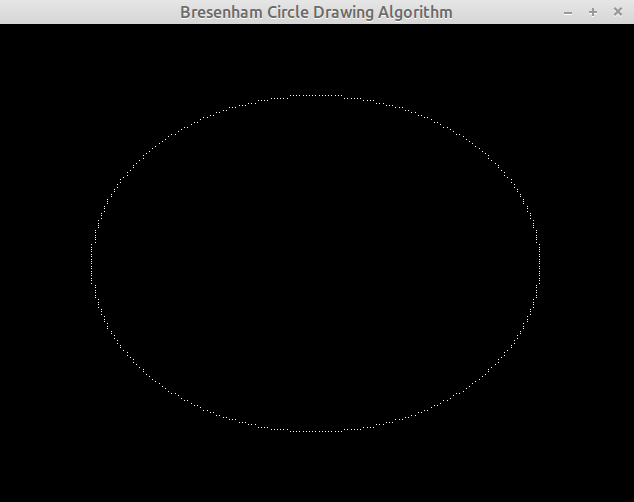
\includegraphics[width=60mm, height=60mm]{circleOpenGL.png}
\caption{Draw circle using bresenhams mid point algo in OpenGL \label{overflow}}
\end{figure}

\begin{figure}[ht!]
\centering
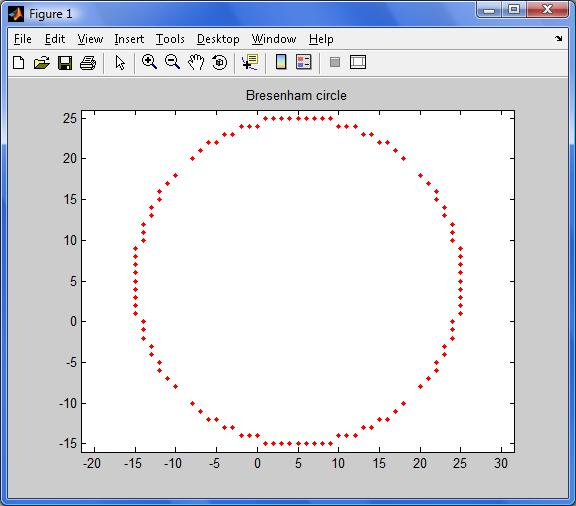
\includegraphics[width=60mm, height=60mm]{circleMatLab.png}
\caption{Draw circle using bresenhams mid point algo in  matlab \label{overflow}}
\end{figure}
\end{document}
